\section{Webserver} \label{sec:Webserver}
Der Webserver bietet die Möglichkeit der Verwaltung des Spiels, der Abgabe von Flags sowie der Durchführung von Käufen im Flagshop und Challenges. Auch können Informationen zum Spiel, wie Einstellungen, Spielstand, Strafen und Teilnehmer abgerufen werden.

\subsection{Verwendung mehrerer Microservices}
Der Webserver kann nach dem Architekturmuster Microservices implementiert werden. Hierbei besteht die Anwendung aus mehreren unabhängig Komponenten, welche, sofern dies notwendig ist, untereinander kommunizieren. Die Komponenten sind so klein wie möglich und können jederzeit durch eine andere Implementierung ausgetauscht werden.\cite{wolffMicroservicesGrundlagenFlexibler2015} 

So wären die verschiedenen Komponenten des Webservers (Flagabgabe, Nutzerverwaltung, Spielsteuerung, etc.) unabhängig von einander und können leichter weiterentwickelt oder ersetzt werden.

Die Verwendung dieses Architekturmuster würde bei der aktuellen Aufgabenstellung zu hohen Aufwand für zu wenig Nutzen bedeuten.

\subsection{Fat Webserver}
Der Webserver beinhaltet sowohl die Logik als auch die Darstellung. Bei einer Anfrage an den Webserver, wird eine Antwort bestimmt und diese dann in eine Vorlage / ein HTML Dokument eingebettet. Danach wird dieses zurück an den Nutzer gesendet.

Während der Implementierung des Prototyps und des weiteren Entwurfs hat sich ein Problem mit dem Flagshop Login herausgestellt.

Für die Nutzung des Flagshops ist ein Multi-Login notwendig, da nur am Webserver eingeloggte Nutzer sich mit einem extra angelegten Account am Flagshop anmelden und diesen verwenden dürfen. Dieses ließ sich mit dem im Prototypen implementierten Session basierten Login nicht einfach umsetzen. 

So ist für diesen Anwendungsfall ein Stateless Login besser geeignet, da hier die benötigten Informationen vom Client, je nach Anliegen, gesendet werden können. 

Die Nutzung des Stateless Logins bietet die Perspektive der Verwendung eines Stateless Webservers sowie eines Thin Webservers. Bei einem Thin Webserver werden nur Daten und keine Repräsentation an dem Client zurückgesendet. So wird die Aufgabe der Darstellung der Daten an den Client übertragen.

Durch die Nutzung eines Thin Servers werden zwei Dinge ermöglicht. 

Zum ersten ist es möglich den Client und Server unabhängig voneinander zu entwickeln, zu verändern und zu verbessern. Damit kann in Zukunft eine Iteration der Software einfacherer geschehen. Zweitens können die Studierenden eigene Clients programmieren, um mit der Anwendung zu interagieren.

\subsection{Thin Webserver}
\begin{center}
	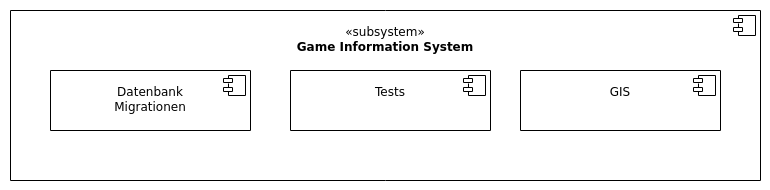
\includegraphics[width=\linewidth]{entwurf/gis/comp-gis}
	\captionof{figure}{Rest Interface im Überblick (Komponentendiagramm)}
\end{center}

Der Server besteht aus der Komponente \textit{Game Information System}, welche wiederum aus drei weiteren Komponenten besteht. 

Die Komponente \textit{GIS} implementiert die gesamte Server Logik. In diesem Modul wird der eigentliche Thin Server, über das die Spieler und Betreuer mit der Anwendung interagieren können, implementiert.

In der Komponente Datenbank Migrationen sind Migrationsskripts hinterlegt, welche die Datenbank Iterationen festhalten. Diese Skripts sollen genutzt werden, um verwendete Datenbanken einfach auf den gleichen Soll-Zustand bringen zu können. 

Die letzte Komponente beinhaltet Unit-Tests. Mithilfe der implementierten Unit-Tests kann die Anwendung bei späteren Änderungen auf Fehler überprüft werden kann.


Da der Thin Server nur eine Brücke zwischen Nutzer und Scanner oder Datenbank darstellt, kann von einer API (Application-Programming-Interface) gesprochen werden. Mithilfe dieser API kann beispielsweise der aktuelle Spielstand aus der Datenbank ausgelesen und Strafen eingetragen werden.

\subsubsection{API}
Um bei der Implementierung der API einem Standard / einem Vorgehen zu folgen, wird der de facto Standard für HTTP-APIs Represntational State Transfer (REST) verwendet.

Ein RESTful Interface ermöglicht, dass Ressourcen auf dem Webserver eindeutig identifizierbar sind, damit diese als Ziel von Operationen ausgewählt werden können. Des Weiteren werden einheitliche Schnittstellen genutzt. Dazu müssen Standardmethoden und -repräsentationen genutzt werden.

Durch diese Anforderungen biete das REST Interface die Möglichkeiten alle zur Verfügung stehenden Ressourcen auf die gleiche Art und Weise zu verwalten. Mit dieser Herangehensweise wird die HTTP Methode GET nicht länger zur Veränderung oder Erschaffung von Ressourcen verwendet, sondern die dafür ausgelegten HTTP-Methoden. Die für die Verwendung benötigten Daten werden auch nicht länger als Paramter der Anfrage beigefügt, sondern im Body der Anfrage übertragen.\cite{beimsWebApplikationenREST2014}

Alle Routen werden mit dem Präfix \textit{/v1} versehen, um bei späteren Iterationen der API Kollisionen zu verhindern und die Nutzung der API v1 weiterhin zu ermöglichen. 

Bei der Implementierung sollen die zur Verfügung stehenden HTTP Methoden benutzt werden. Das Rest-Interface soll auch mit entsprechenden HTTP Codes antworten, um die Antwort und den Erfolg einer Anfrage auch ohne Antworttext interpretieren zu können. Bei der Datenübertragung zwischen Client und Server soll das JavaScript Object Notation (JSON) Format für die Formatierung der gesendeten Daten verwendet werden.

\begin{table}
	\centering
	\begin{tabular}{c c}
		GET & Auf Ressourcen zugreifen \\ 
		POST & Neue Ressourcen erzeugen \\  
		PUT & Bestehende Ressourcen verändern \\
		DELETE & Vorhandene Ressourcen löschen \\
	\end{tabular}
	\caption{Übersicht über die verwendeten HTTP Methoden}
	\label{table:http-methods}
\end{table}

Neben den in Tabelle \ref{table:http-methods} aufgezeigten Methoden gibt es noch weitere HTTP Methoden, welche keine Anwendung in dem zu implementierenden Rest-Interface erhalten.

\begin{table}
	\centering
	\begin{tabular}{l l}
		Route									 & Methods \\ [0.5ex]
		\hline
		/										 & GET \\
		/associate								 & GET, POST \\
		/associate/<int:associate\_id>			 & DELETE \\
		/auth/flagshop/login					 & POST \\
		/auth/login								 & POST \\
		/auth/refresh							 & POST \\
		/auth/revoke/access						 & DELETE \\
		/auth/revoke/refresh					 & DELETE \\
		/backup									 & GET \\
		/backup/<int:backup\_id>				 & GET \\
		/challenge								 & GET, POST \\
		/challenge/<int:challenge\_id>			 & DELETE, GET, PUT \\
		/challenge/solve						 & GET \\
		/challenge/solve/<int:challenge\_id>	 & DELETE, POST \\
		/client									 & GET, POST \\
		/client/<int:group\_id>					 & DELETE, GET \\
		/flag									 & POST \\
		/flagshop/package						 & GET, POST \\
		/flagshop/package/<int:package\_id>		 & DELETE, PUT \\
		/flagshop/transaction					 & DELETE, GET, POST \\
		/flagshop/user							 & GET, POST \\
		/flagshop/user/<user\_name>				 & DELETE, PUT \\
		/log									 & GET, POST \\
		/log/old								 & GET \\
		/match/control							 & DELETE, POST, PUT \\
		/match/info								 & GET \\
		/match/score							 & GET \\
		/note									 & GET, POST \\
		/note/<int:note\_id>					 & DELETE, GET, PUT \\
		/penalty								 & GET, POST \\
		/penalty/<int:penalty\_id>				 & DELETE, GET, PUT \\
		/scanner								 & DELETE, GET, POST \\
		/scanner/notify							 & POST \\
		/secure									 & GET \\
		/service								 & GET \\
		/service/<int:service\_id>				 & DELETE, GET, PUT \\
		/setting								 & GET, PUT \\
		/user									 & DELETE, GET, POST \\
		/user/<int:user\_id>					 & DELETE, GET, PUT \\
		/user/import							 & POST \\
	\end{tabular}
	\caption{Übersicht über die zu implementierenden Routen}
	\label{table:gis-routes}
\end{table}


(todo: Module / Komponenten des REST-Interface)
\paragraph{Authentifizierung}

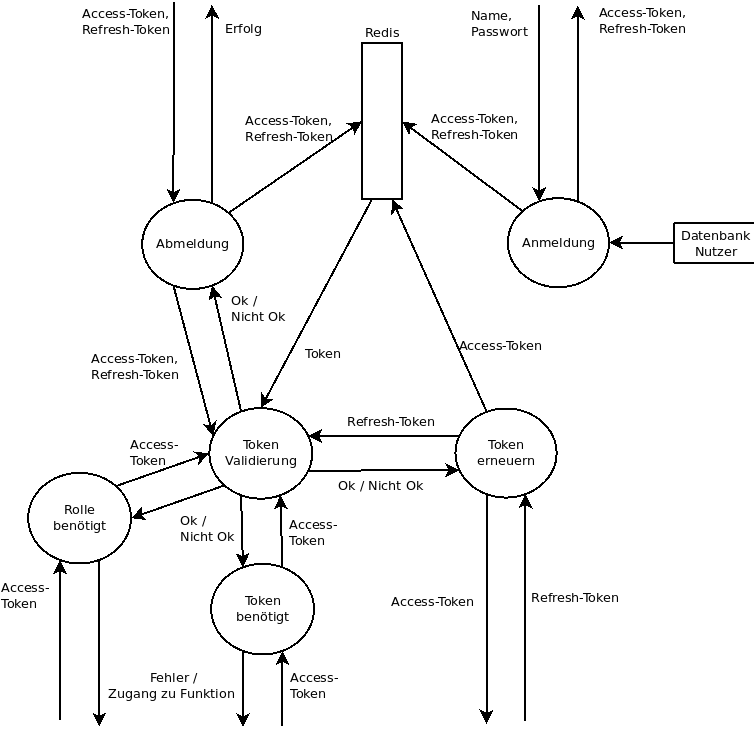
\includegraphics[width=\linewidth]{entwurf/gis/dfd-watchdog-security}
\captionof{figure}{Datenfluss in der Security Komponente (Datenflussdiagramm)}

\paragraph{Flaggengenierung}
- Änderung des Algo
- Änderung des Vorgehens -> Generierung auf dem Server -> Versand an den Client (Secret nicht auf dem Client, Abfangen aller Flags möglich, Verschlüsselung bringt nix, da Nutzer root Rechte hat)

\paragraph{Challenges}
todo:
Challenge Informationen und Lösung der Challenge über API, Darstellung / Inhalt der Challenge über anderen Webserver (da wo auch der Webclient ausgelieftert wird), da gedanke ist nur Daten zu übertragen und keine HTML Seiten etc.

\subsection{Reverse Proxy}
Für das Betreiben wird auf den bereits im EZS Labor verwendeten Apache HTTP-Server zurückgegriffen. Durch die Entscheidung bleibt dieser als einziger als Einstiegspunkt für Anfragen zuständig. Des Weiteren wird die Protokollierung der Anfragen sowie die Verschlüsselung der Verbindung an die Webserver Software abgegeben.

Der Reverse Proxy muss bei der Weiterleitung der Anfrage an das GIS die eigentliche IP-Adresse der Anfrage weiterleiten. Dieses wird benötigt um die IP-Adresse, und so die zugehörige Gruppe, bei der Registrierung und dem Login zu bestimmen. Die originale IP-Adresse der Anfrage soll in einen HTTP Header gespeichert werden.

In einen HTTP Header können Server und Client zusätzliche Informationen zur Anfrage oder Antwort beifügen.\cite{mdncontributorsHTTPHeaders2020}

Um einen Spoofing-Angriff zu erschweren und das Vertrauen in den Header mit der IP-Adresse zu erhöhen, soll ein weiterer Header mit einem Geheimnis gesetzt werden. Anhand dieses kann das GIS entscheiden, ob die Anfrage über einen vertrauenswürdigen Proxy weitergeleitet oder ob ein Spoofing-Angriff durchgeführt worden ist. Die Erweiterung wird benötigt, da die Anwendung auch ohne einen Reverse Proxy betrieben werden kann. In diesem Anwendungsfall kann die angreifende Person sich als Proxy für eine andere Gruppe ausgeben.

Bei einem Spoofing-Angriff versendet die angreifende Person Anfragen für andere IP-Adressen und erhält die Antwort. So kann dieser im Namen anderer agieren und diesen beispielsweise Minuspunkte verschaffen.